
% \addbibresource{./references.bib}

This section we will mainly discuss our measurement about memory performance on the target machine. More specificly, we will report measurements about access latency on each level of memory hirachy, the memory bandwidth, and the overhead of page fault handling.

\subsection{Memory Latency}

\subsubsection{Methodology}

When measure access latency on each level of memory hirachy, basically we followed the method suggest by lmbench\cite{mcvoy1996lmbench}.

We create a linklist which only contains a pointer to the next element:

\begin{lstlisting}
    struct Linklist {
        struct Linklist * next;
    };

    typedef struct Linklist Linklist;
\end{lstlisting}

The total size of the linklist will increase from 1 KB to 256 MB, by the factor of 2. When initializing, a stride will be provided by the tester. The number of the elements in the linklist is always divisible by the stride, and when initializing, the linklist will be devided as many chunks contains stride elements, and each elements in one chunk will point to a random element in the next chunk, and the last chunk in the linklist element array will point to the first chunk, which make this linklist an infinite cyclical linklist. This structure will eliminate the impact of cache prefetch, as the stride and random elements can easily make the next element in the linklist out of the prefetch range of each level of cache.

When performing measurement, in order to get rid of all other unnecessary memory access, we have to use at least \textbf{O1} optimization; however, \textbf{O1} optimization will also optimized the code accesing the linklist. In our final measurement code, the travel of the linklist if write in inline assembly which can avoid compiler optimizations:

\begin{lstlisting}[language=C]
    START_COUNT(high, low);
    while (step --> 0) {
#define INST "movq	(%%rax), %%rax\n\t"
        asm volatile ("mov %0, %%rax\n\t" \
                       HUNDRED(INST) \
                       "mov %%rax, %1"
                       : "=r" (iter)
                       : "r" (iter)
                       : "%rax");
    }
    STOP_COUNT(high1, low1);
\end{lstlisting}

where iter is the head of the linklist. We will measure 100 times of accesing memory on each measurement, and totally perform 1000 (stored in \textbf{step}) measurements.

\subsection{Estimation and Results}

\begin{figure}[ht]
    \centering
    \frame{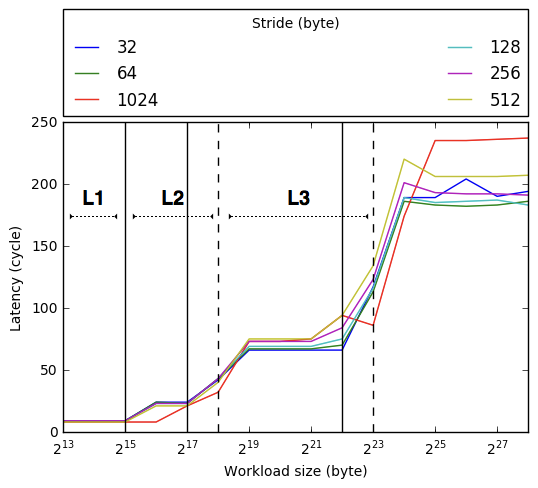
\includegraphics[width = .9\textwidth]{pictures/memLatency.png}}
    \caption{Memory Hirachy Latency: Estimation and Experiment Results }
    \label{mem_latency_result}
\end{figure}

\begin{table}[ht]
  \centering
  \caption{\textbf{Memory Hirachy Latency: Estimation and Experiment Results}}
  \begin{threeparttable}
  \begin{tabular}{ccc}
  \hline
      \textbf{Memory}    & \textbf{Latency}   & \textbf{Expr. Results} \\
      \textbf{Hiracht}   & \textbf{Estimation}  & (AVG)   \\
  \hline
      \textbf{L1}  & 5 cycles & 9 cycles   \\
      \textbf{L2}  & 20 cycles & 20 cycles   \\
      \textbf{L3}  & 60 cycles & 70 cycles   \\
      \textbf{L4}  & 150 cycles & 190 cycles   \\
  \hline
  \end{tabular}
  \end{threeparttable}
  \label{memory_latency_table}
\end{table}

For estimation, we believe the latency for l1 cache references should be pretty low, let's say, within 5 cycles; the latency for l2 cache should be higher, let's say, 20 cycles; the latency for l3 cache should be much higher than l2, let's say, 60 cycles; and the latency for main memory should be the highest and much higher than l3 cache, let's say, 150 cycles.

The result is shown in \textbf{Figure \ref{mem_latency_result}} and \textbf{Table \ref{memory_latency_table}}. In \textbf{Figure \ref{memory_latency_table}}, the real lines separate the latency turning point for different level of memory hirachy, and the dotted lines separate the real size of different level of memory hirachy in the target machine. As we can see in the figure, the dotted line and the real line for l1 cache is on the same position, but for l2 cache and l3 cache, the latency turning point is always a little bit smaller than the actual size point. For why that happened, we guess that the following reason contribute it: as both l2 and l3 cache are unify instruction and data cache, so that some instructions stored in the l2 cache and l3 cache will accelarate that data access latency turning point to happen.

\textbf{Table \ref{memory_latency_table}} shows the latency esitimation and measurement results. We under estimate the access latency of l1 cache and memory.

\subsection{Memory Bandwidth}

\subsubsection{Methodology}

When measuring memory bandwidth, we used \textbf{memcpy()} function, to copy a large chunks of data (same size as l3 cache) from main memory to l3 cache when measuring read bandwith, or to copy a large chunks of data (same size as l3 cahce) from l3 cache to main memory when measuring write bandwidth. When calculating the results, we made an assumption that, only around a half of the overhead of \textbf{memcpy()} is caused by main memory reading or writing, as \textbf{memcpy()} itself will perform a lot of protection and validation operations. We believe that it is reasonable to assume that around a half of the overhead is caused by desired memory accesing.

\subsubsection{Estimation and Results}

\begin{table}[ht]
  \centering
  \caption{\textbf{Memory Bandwidth: Estimation and Experiment Results}}
  \begin{threeparttable}
  \begin{tabular}{ccccc}
  \hline
      \textbf{Read or} & \textbf{Bandwidth}   & \textbf{Expr. Results} & \textbf{Standard}\\
      \textbf{Write}   & \textbf{Estimation}  & (AVG)   & \textbf{Deviation} \\
  \hline
      \textbf{Read}  & 10600 MB/s & 9356.70657557 MB/s & 336.209601362  \\
      \textbf{Write} & 10600 MB/s & 8364.93322737 MB/s & 500.236423781  \\
  \hline
  \end{tabular}
  \end{threeparttable}
  \label{memory_bandwidth_table}
\end{table}

For estimation, Frank Denneman stated on his web blog \cite{frankdenneman} that, the bandwidth for both reading and writing of a DDR3-1333 memory is 10600 MB/s, we take this as our estimation.

The measurement result is shown in \textbf{Table \ref{memory_bandwidth_table}}. The results shows that memory reading bandwidth should be \textbf{9356.71 MB/s}, and writing bandwidth should be \textbf{8364.93 MB/s}. Measurement result is slightly below the estimation value, we think the reason for that is:

First, although we estimate that, the memcpy will copy all data from main memory to l3 cache only for reading measurement, and from l3 cache to main memory only for writing measurement, there is possibility that l3 cache cached address not in the target range for measurement right before memcpy, so that l3 cache replacement needed when memcpy data, which will cause additional overhead;

Second, we might under estimated the software overhead (we estimate as half of total overhead when doing measurement), which will cause the measurement result a little bit smaller than the actual value. However, as we are not sure how \textbf{memcpy()} implement, it is impossible for us to accurately estimate the software overhead of \textbf{memcpy()}.

The writing bandwidth is smaller than reading bandwidth, as \textbf{Table \ref{memory_bandwidth_table}} shown. This is reasonable, as writing do be slower than reading for DRAM.

\subsection{Page Fault Handling}

\subsubsection{Methodology}

When measuring page fault handling overhead, we will first create a large file (40 MB) on disk, then using \textbf{mmap()} system call, to map the file into the main memory. Then, we will reading data in that file, as \textbf{mmap()} only mapping that file into destination memory chunks, not reading file contents into main memory, the reading operation will cause a page fault. The operating system will handle that page fault, and that's what we want to measure.

There is still one problem needs to be addressed out, the file system optimization. The file system will cache the contents of the file and also perform file prefetch from the disk, so that, if we failed to bypass those optimization, we could not accurately measure the page fault handling overhead. To bypass those optimization, the measurement program will access the file with a stride applied with a random offset on page.

\subsubsection{Estimation and Results}

\begin{table}[ht]
  \centering
  \caption{\textbf{Pagefault Handling Overhead: Estimation and Experiment Results}}
  \begin{threeparttable}
  \begin{tabular}{cccccc}
  \hline
        \textbf{HW Overhead} & \textbf{SW Overhead } & \textbf{Total Overhead} & \textbf{Expr. Results} & \textbf{Standard}\\
        \textbf{Estimation}       &  \textbf{Estimation}         & \textbf{Estimation}  & (AVG)   & \textbf{Deviation} \\
  \hline
        111600 cycles & 10000 cycles & 121600 cycles  & 136875.058065 cycles & 13433.5243954 \\
  \hline
  \end{tabular}
  \end{threeparttable}
  \label{pagefault_handle_time}
\end{table}

For estimation, the I/O speed of a 7200 RPM HDD is at the scale of 100 MB/s \cite{wiki:hdd}, so that transfering a 4K page will take:

$$ \frac{4KB}{100 MB/s} = \frac{1}{25600} s $$

$\frac{1}{25600} s$ equals to around $111600 cycles$.

The software overhead mainly comes from page table maintains and protection mechanism, and we assume this overhead is around 10000 cycles. Then, the total estimation overhead for a pagefault handling is 121600 cycles.

The result is shown in \textbf{Table \ref{pagefault_handle_time}}. We underestimate the overhead of the pagefault handling by around 15000 cycles. This might be caused by two reasons: first, we might underestimate software overhead caused by Operating System's handling logic; second, the I/O speed of the HDD might not reach its theorical speed.

For the question about speed compare between memory bandwidth and page fault page transfer bandwidth on byte scale, on average, the memory can transfer a byte in

$$\frac{1 Byte}{9356.70657557 MB/s} = 0.101924 ns $$

and the page fault mechanism can transfer a byte in

$$\frac{1 Byte}{\frac{4 KB}{136875 cycles} * \frac{1}{0.358001 ns/cycle}} = 11.963229 ns $$.

Thus the page fault handling is more than 100 times more expensive than a page hit memory access.
